%%%%%%%%%%%%%%%%%%%%%%%%%%%%%%%%%%%%%%%%%%%%%%%%%%%%%%%%%%%%
%%% ELIFE ARTICLE TEMPLATE
%%%%%%%%%%%%%%%%%%%%%%%%%%%%%%%%%%%%%%%%%%%%%%%%%%%%%%%%%%%%
%%% PREAMBLE 
\documentclass[9pt,lineno]{elife}
% Use the onehalfspacing option for 1.5 line spacing
% Use the doublespacing option for 2.0 line spacing
% Please note that these options may affect formatting.
% Additionally, the use of the \newcommand function should be limited.

\usepackage{lipsum} % Required to insert dummy text
\usepackage[version=4]{mhchem}
\usepackage{siunitx}
\DeclareSIUnit\Molar{M}

%%%%%%%%%%%%%%%%%%%%%%%%%%%%%%%%%%%%%%%%%%%%%%%%%%%%%%%%%%%%
%%% ARTICLE SETUP
%%%%%%%%%%%%%%%%%%%%%%%%%%%%%%%%%%%%%%%%%%%%%%%%%%%%%%%%%%%%
\title{Engineering another (better) biosensor for aspartate}

\author[1,2,\authfn{1}]{Kristian Davidsen}
\author[3,\authfn{1}*]{Jonathan S Marvin}
\author[3]{Tim Brown}
\author[1*]{Lucas B Sullivan}
\affil[1]{Human Biology Division, Fred Hutchinson Cancer Center, Seattle, WA, USA}
\affil[2]{Molecular and cellular biology program, University of Washington, Seattle, WA, USA}
\affil[3]{Howard Hughes Medical Institute (HHMI), Janelia Farm Research Campus, Ashburn, VA, USA}

\corr{marvinj@janelia.hhmi.org}{JSM}
\corr{sullivan@fredhutch.org}{LBS}

\contrib[\authfn{1}]{These authors contributed equally to this work}

%%%%%%%%%%%%%%%%%%%%%%%%%%%%%%%%%%%%%%%%%%%%%%%%%%%%%%%%%%%%
%%% ARTICLE START
%%%%%%%%%%%%%%%%%%%%%%%%%%%%%%%%%%%%%%%%%%%%%%%%%%%%%%%%%%%%

\begin{document}

\maketitle

\begin{abstract}
Aspartate is an important metabolite in the biology of cancer cells, derived primarily from action of glutaminase on glutamine, and subsequent conversion to aspartate.
Detection of aspartate has primarily been from mass spectrometry, which is limited by its spatial and temporal resolution.
We have developed multiple generations and variants of intensity-based glutamate sensing fluorescent reporters (iGluSnFRs), which have proven useful for studying glutamate release from neurons in vivo. iGluSnFRs also bind aspartate, but with higher Kd.
To make an intensity-based aspartate sensing fluorescent reporter, we made two mutations to an iGluSnFR3 variant, resulting in a sensor with 50 µM affinity for aspartate, > 5 mM affinity for glutamate and asparagine, with an over 20-fold total increase in fluorescence upon saturation with aspartate.
We validate the sensors ability to quantify the concentration of aspartate in cells by correlating fluorescence to mass spectrometry results, and then use the sensor to resolve temporal changes in intracellular aspartate using both genetic and pharmacological manipulations.
\end{abstract}


\section{Introduction}
The primary tool used by metabolism researchers, liquid chromatography coupled with mass spectrometry (LCMS), involves extracting pools of thousands of cells and measuring the liberated metabolites.
This approach is powerful but has significant drawbacks; it requires highly specialized equipment, it is expensive for use, and sample preparation by chemical extractions homogenizes metabolic differences that may occur amongst different cells in complex samples or across subcellular compartments.
Metabolite extraction also consume precious samples that might otherwise be desirable to analyze over time or with additional outputs.
Development of genetically encoded protein sensors (biosensors) over the past two decades has provided new opportunities to visualize the release, production, and depletion of important signaling molecules and metabolites with subsecond and subcellular resolution (reviewed in \cite{Kostyuk2019-qc, Koveal2020-cl}).
Thus, biosensors provide a solution to many of the problems with metabolite extraction and LCMS, however; at the price of monitoring only one metabolite per sensor.

Aspartate is amongst the most concentrated metabolites in cells [ref], yet it is one of only two amino acids that is not predominantly acquired from the environment.
While the other, glutamate, is made from glutamine by the enzyme glutaminase, no analogous enzyme exists in humans to convert asparagine to aspartate [refs].
Instead, aspartate must be synthesized by transamination of tricarboxylic acid (TCA) cycle metabolite oxaloacetate by the cytosolic enzyme GOT1 or the mitochondrial enzyme GOT2.
Notably, aspartate synthesis can occur from multiple metabolic sources via complex metabolic reactions occurring in the mitochondria and cytosol, rendering aspartate levels at the whole cell and subcellular levels dependent on multiple metabolic variables [refs].
For example, impairments to mitochondrial respiration can deplete aspartate levels and aspartate restoration can reestablish proliferation in cells with defective mitochondria [references].
Alterations to aspartate levels can also modify cell function in multiple biological processes, including stem cells [ref], immune cells [ref], and endothelial cells [ref], and others [ref].
In addition, genetic methods to elevate intracellular aspartate can impact biology in vivo, increasing tumor growth [refs] and improving hematopoietic function [ref].
Therefore, the understanding of metabolism could be improved with the availability of an aspartate biosensor. 

We have previously developed a biosensor for glutamate using the E.coli glutamate/aspartate binding domain GltI linked to circularly permutated GFP (iGluSnFR) \citep{Marvin2013-qq}, and subsequently optimized it by modulating its affinity, kinetics, color, and total fluorescence change (iGluSnFR3) \citep{Marvin2018-ks, Aggarwal2023-pi}.
Since mutations to the GltI domain can confer glutamate specificity, we reasoned that suitable mutations could also infer aspartate specificity.
We achieved this using a small mutagenesis screen on iGluSnFR3, guided by the crystal structure of glutamate bound GltI. The resulting biosensor, iAspSnFR, was then characterized biochemically and in cells with matched LCMS determination of aspartate, showing that it accurately reports genetic and pharmacological modulation of intracellular aspartate.




\section{Results}

\subsection{Protein engineering}
We observed that original iGluSnFR bound both glutamate and aspartate, with higher affinity for the former \citep{Marvin2013-qq}, as expected from previous identification of GltI \citep{Hu2008-nd}.
To shift the relative affinities of the two ligands, we looked at the structure of the binding pocket and sampled all possible amino acid substitutions of residue S72, which interacts with the OE1 and OE2 of bound glutamate.
By simply expressing mutant sensors in bacteria and measuring the fluorescence of bacterial lysate in response to aspartate or glutamate, we identified S72A and S72P as having switched aspartate/glutamate specificity.
S72T, identified in a faster version of iGluSnFR \citep{Helassa2018-fb} also preferably binds aspartate over glutamate. 

As iGluSnFR3 was being developed \citep{Aggarwal2023-pi}, we took a variant from that process and queried the effect of S72A, S72T, and S72P on aspartate/glutamate affinity.
In bacterial cell lysate, S72P maintained the expected shift to a preference for aspartate, and had a higher ∆F/F than either S72A or S72T (Supp Fig S1a).
To further separate the aspartate/glutamate specificity, we sampled mutations at S27, which also interacts with OE1 and OE2 of bound glutamate, in the background of S72P.
One of those, S27A, had even lower affinity for Glut (Supp Fig S1b). We named this variant iAspSnFR. Since we expected to be using this sensor in cell culture studies, and potentially in vivo, over the course of hours or even days, we included a C-terminal red fluorescence protein, mRuby3, to correct for expression and movement artefacts. All data reported are with iAspSnFR.mRuby3.

The sensor is yellow-shifted in excitation and emission from typical GFP-based sensors (Supp Fig S1c), since its chromophore is formed by the triad of GYG and has the T203Y pi-stacking mutations of Venus.
This yellow-shift will facilitate observation deeper into tissues using 2-photon microscopy, as the sensor has high ∆F/F and significant 2-photon cross-section at 1040 nm (Supp Fig S1c).
It has a Kd for aspartate of about 50 µM and binds glutamate and asparagine with Kd greater than 5 mM (Fig 1b). It does not appreciably change its green fluorescence in response to other amino acids (Supp Fig S1d).
Surprisingly, the mRuby3 component responds to all amino acids at high millimolar concentrations, indicating a non-specific effect (potentially interacting with the C-terminal histidine tag) (Supp Fig S1e), although this increase in fluorescence is still an order of magnitude lower than the green fluorescence response.
The sensor does not respond to other decoys considered relevant to aspartate metabolism nor to relevant pharmacological treatments (Supp Fig S1f). Unlike a recently reported sensor for aspartate [https://www.biorxiv.org/content/10.1101/2023.05.04.537313v1], our iAspSnFR responds to aspartate at 37°C with slightly higher ∆F/F than at 23°C (Supp. Fig S1g).
It is sensitive to pH, as are all cpGFP-based sensors, but changes in fluorescence due to changes in [aspartate] far exceed what one might expect from changes in fluorescence due to changes in pH (Supp Fig S1h).


\subsection{iAspSnFR reveals the temporal dynamics of aspartate limitation}
\lipsum[5]




\subsection{Steady-state iAspSnFR signal correlates with intracellular aspartate concentration}
\lipsum[7]


And look here is a duck \FIG{fig1}.






\begin{figure}[ht!]
\centering
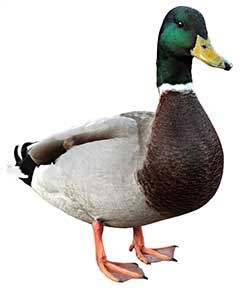
\includegraphics[height=2cm]{figures/duck.jpg}
\caption{
First figure: method summary, oligo design (maybe just illustrations)
}
\label{fig:fig1}
\end{figure}


\begin{figure}[ht!]
\centering
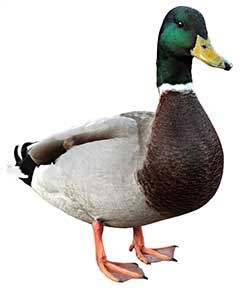
\includegraphics[height=2cm]{figures/duck.jpg}
\caption{
Second figure: method optimization, improved Whitfeld reaction, ligation completion etc. (mostly gel images)
}
\label{fig:fig2}
\end{figure}

\figsupp[Shorter caption for main text.]
{This is a supplementary figure's full caption, which will be used at the end of the manuscript. 
  \figsuppdata{A data source; see \url{https://doi.org/xxx}}
  \figsuppdata{Another data source.}
  \figsuppsrccode{And the source code.}}
{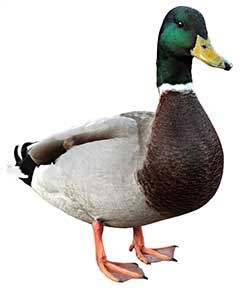
\includegraphics[width=6cm]{figures/duck.jpg}}\label{figsupp:sfig2_1}

\figsupp[Shorter caption for main text.]
{This is a supplementary figure's full caption, which will be used at the end of the manuscript. 
  \figsuppdata{A data source; see \url{https://doi.org/xxx}}
  \figsuppdata{Another data source.}
  \figsuppsrccode{And the source code.}}
{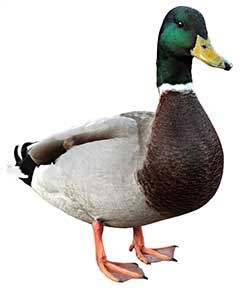
\includegraphics[width=6cm]{figures/duck.jpg}}\label{figsupp:sfig2_2}






\begin{figure}[ht!]
\centering
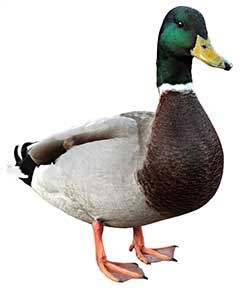
\includegraphics[height=2cm]{figures/duck.jpg}
\caption{
Third figure: alignment optimization, comparison to Behrens, coverage and mutation plots etc.
}
\label{fig:fig3}
\end{figure}














\section{Discussion}
Other/future uses for the sensor.

Compare to other paper:
They have different Asp/Glu affinities; higher Asp (probably higher than relevant low levels) but also very high Glu (thus great specificity). Temperature is not an issue with our sensor, fold change also appear higher.
DMS screening is necessary to achieve the goal of switching substrate specificity; sensitivity and specificity can be modulated in ways predictable from crystal structure. Our rational design only required two mutations. While not necessary for switching substrate specificity in this case, DMS is in important tool for protein engineering and potentially switching the substrate specificity beyond what can be tested using low throughput rational design.

Apparent Asp affinity is higher in cells than in lysate. Probably, Asp is bound by other proteins in the cell.

General caveats of biosensors (French mito temperature sensor disaster is a good example). Cell line sensitive, not measuring concentration, sensitivity in a limited (smaller) concentration range, pH sensitive (mito use), generally sensitive to a plethora of possible external factors and thus should always be used with caution.

Room for development:
Sometime we encounter better expression of the non-RFP fused sensor.










\section{Methods and Materials}

\subsection{Sensor engineering}
Parent construct, sites mutated, expression vector etc.


\subsection{Protein expression and purification}
Maybe unnecessary because it is included under biochemical characterization.


\subsection{Sensor biochemical characterization}
Metabolite titrations, pH and temperature, ex/em spectra, reagents, instrumentation etc.





\subsection{Cell culture}
Cell lines were acquired from ATCC (HEK293T, H1299, HT1080) and tested to be free from mycoplasma (MycoProbe, R\&D Systems).
Cells were maintained in Dulbecco’s Modified Eagle’s Medium (DMEM) (Gibco, 50-003-PB) supplemented with 3.7 g/L sodium bicarbonate (Sigma-Aldrich, S6297), 10\% fetal bovine serum (FBS) (Gibco, 26140079) and 1\% penicillin-streptomycin solution (Sigma-Aldrich, P4333).
Cells were incubated in a humidified incubator at 37°C with 5\% CO2.

\subsection{Generation of nuclear RFP cell lines}
Nuclear expressing cell lines were generated using 1e5 transducing units of EF1A-nuclear RFP lentivirus (Cellomics Technology, PLV-10205-50) by spinfection.
Cells were seeded at 50\% confluency in 6 well dishes and lentivirus was added to fresh media with 8 µg/µL polybrene and added to cells followed by centrifugation (900g, 90 mins, 30°C).
Two days after infection, cells were sorted for high RFP expression using fluorescence-activated cell sorting (FACS).
High RFP cells were then expanded and single-cell cloned by limiting dilution, plating 0.5 cells/well on a 96 well plate.
Plates were then screened for RFP expression and localization using Incucyte S3 (Sartorius) and a suitable clone chosen, expanded, and used for all subsequent experiments. 

\subsection{Lentiviral production and stable cell line generation}
iAspSnFR and iAspSnFR-RFP (iASPSnFR with a C-termal fusion to mRuby) were first cloned into entry vector pENTR1A (Fisher, A10462) using NEBuilder HiFI DNA Assembly Cloning Kit (New England BioLabs, E2621).
These donor constructs were then used to transfer their insert into destination vectors: pLX304-CMV-Blast (Addgene, 25890), pLenti-CMV-Hygro (w117-1) (Addgene, 17454 a gift from Eric Campeau \& Paul Kaufman), or pLX304-CAG-Blast using LR Clonase II (Fisher, 11791100).
pLX304-CAG-Blast was generated in house by swapping the CMV promoter region of pLX304-CMV-Blast with a CAG promoter provided on synthetic DNA (Integrated DNA Technologies).
Each plasmid sequence was verified by whole plasmid sequencing (Plasmidsaurus).
Lentivirus was generated by transfection of HEK293T cells with destination vectors plasmid DNA with the packaging plasmids pMDLg/pRRE (Addgene, 12251), pRSV-Rev, (Addgene, 12253) and pMD2.G (Addgene, 12259) and FuGENE transfection reagent (Fisher, PRE2693) in DMEM (Fisher, MT10017CV) without FBS or penicillin-streptomycin.
The supernatant containing lentiviral particles was filtered through a 0.45 µM membrane (Fisher, 9720514) and was supplemented with 8 µg/µL polybrene (Sigma, TR-1003-G) prior to infection.
For infection, cells were seeded at 50\% confluency in 6 well dishes and centrifuged with lentivirus (900g, 90 mins, 30°C).
After 24 hours the media was replaced with fresh media and after 48 hours cells were treated with either 1 µg/mL blasticidin (Fisher, R21001) or 150 µg/mL hygromycin (Sigma-Aldrich, H7772-1G) and maintained in selection media until all uninfected control cells died.
After selection, cells were expanded and single-cell cloned by limiting dilution, plating 0.5 cells/well using 2-3 96 well plates. These clones were incubated until 10-30\% confluency and screened for high GFP and RFP signal using Incucyte S3 (Sartorius).
The highest expressing monoclonal cells were selected and further expanded on 6 well plates and screened for fluorescence using the Incucyte.
Clones were then expanded and used for subsequent experiments.
Different cell lines received different vector-sensor combinations: HEK293T cells were infected with pLX304-CAG-Blast-iAspSnFR-RFP, HT1080 with pLenti-CMV-Hygro-iAspSnFR-RFP and HT1080, H1299 and H1299 GOT1/2 DKO cells expressing nuclear RFP were infected with pLenti-CMV-Hygro-iAspSnFR.

\subsection{Generation of GOT1/2 double knockout (DKO) cells}
Protocol and guide RNA generation was identical to that described in \cite{Hart2023-gp}.
Briefly, three chemically synthesized 2'-O-methyl 3’phosphorothioate-modified single guide RNA (sgRNA) sequences targeting GOT1 and GOT2 were purchased (Synthego), sgRNA sequences are shown in the table below.
A pool of six sgRNAs for GOT1 and GOT2 were resuspended in nuclease-free water, combined with SF buffer (Lonza, V4XC-2032), and sNLS-spCas9 (Aldevron, 9212). 2x105 H1299 cells were resuspended in the resulting solution containing ribonucleoprotein complexes (RNPs) and electroporated using a 4D-Nucleofector (Amaxa, Lonza).
Nucleofected cells were then expanded and single-cell cloned by limiting dilution by plating 0.5 cells/well in a 96 well plate.
Gene knockout was confirmed using western blots.

\begin{table}[h!]
\caption{\label{tab:guides}CRISPR guides}
\begin{tabular}{|l|l|}
\hline
Gene & sgRNA   sequence (5’-3’) \\
\hline
GOT1 & \begin{tabular}[c]{@{}l@{}}\texttt{CAGUCAUCCGUGCGAUAUGC}\\\texttt{GCACGGAUGACUGCCAUCCC}\\\texttt{CGAUCUUCUCCAUCUGGGAA}\end{tabular} \\
\hline
GOT2 & \begin{tabular}[c]{@{}l@{}}\texttt{UUUCUCAUUUCAGCUCCUGG}\\\texttt{CGGACGCUAGGCAGAACGUA}\\\texttt{UCCUUCCACUGUUCCGGACG}\end{tabular} \\
\hline
\end{tabular}
\end{table}


\subsection{Intracellular iAspSnFR measurements}
Experiments were conducted in DMEM without pyruvate (Corning 50-013-PB) supplemented with 3.7 g/L sodium bicarbonate 10\% dialyzed fetal bovine serum (FBS) (Sigma-Aldrich, F0392) and 1\% penicillin-streptomycin solution.
To start an experiment, cells were trypsinized (Corning, 25051CI), resuspended in media, counted using a coulter counter (Beckman Coulter, Multisizer 4) and seeded onto 24-well dishes (Nunc, 142475) with an initial seeding density of 50,000, 70,000, 70,000 or 150,000 cells/well for H1299, H1299 GOT DKO, HT1080 and HEK293T, respectively. After 24h (H1299, HT1080, HEK293T) or 48h (H1299 GOT DKO) incubation treatment was added and plates moved into an Incucyte S3 (Sartorius) live cell imaging platform inside a humidified incubator at 37°C with 5\% CO2. Rotenone (Sigma-Aldrich, R8875), metformin (Sigma-Aldrich, D150959) and antimycin A (Sigma-Aldrich, A8674) treatments were spiked-in as 20x solutions in water and the 2 mM pyruvate (Sigma-Aldrich, P8574) was added as 1000x stock.
For treatments with varying media aspartate (Sigma-Aldrich, A7219) or glutamine (Sigma-Aldrich, G5792), wells were thrice washed and filled with media deplete of the given amino acid, then it was added as a spike-in at the specified concentration as 20x solutions in water.
For plates receiving asparagine (Sigma-Aldrich, A7094), this was added to 1 mM from as 20x solution in water, with vehicle wells receiving water.
Live cell imaging was performed on the Incucyte S3 using the GFP and RFP channels with default exposure times.
Images were processed using the associated Incucyte software to subtract background, define areas of cell confluence and GFP/RFP signal and extract the sum of the fluorescence signal in these areas.
The data for the GFP signal, RFP signal, GFP/RFP ratio and confluence for each well at each timepoint was exported and used for further data processing using Python code.
The iAspSnFR signal (GFP channel) was normalized to an RFP signal, either as a stably expressed nuclear localized RFP or mRuby C-term fusion to iAspSnFR.
For temporal measurements the first scan was made 30 min after treatment with subsequent scans indicated on relevant plots.
For some experiments a pre-treatment scan was made shortly prior to treatment to normalize the data to this point.
For comparisons of steady-state measurements of GFP/RFP versus mass spectrometry based metabolite measurements, a single scan was made 24h after treatment, the plate was then quickly moved to ice and metabolite extraction performed (see below).
Another plate was processed in parallel for cell volume determination using a coulter counter and averaging across three replicate wells.
The normalized iAspSnFR signal as a function of intracellular aspartate concentration (c) was fitted by a modified Hill curve:

$$
f(c) = t + \frac{b - t}{1 + (c/m)^s}
$$

With $t$, $b$ being the top and bottom of the curve, respectively, describing the upper and lower asymptotes of normalized iAspSnFR signal.
The curve slope is described by $s$, also known as Hill coefficient, and the midpoint ($m$) describes the intracellular aspartate concentration at half maximum iAspSnFR signal.
The curve parameters were fitted to the data using the Broyden–Fletcher–Goldfarb–Shanno (BFGS) algorithm with an upper bound constraint on the top of the curve of 1.2 times the maximum observed normalized iAspSnFR signal in any of the conditions on the same plot.

\subsection{Metabolite extraction}
For polar metabolite extraction, a plate was move to ice and the media was thoroughly aspirated.
For H1299 and HT1080 cells, wells were washed once with cold saline (Fisher, 23293184).
For HEK293T cells, washing was omitted due to weak cell adherence. Then, 1 mL 80\% HPLC grade methanol in HPLC grade water was added, cells were scraped with the back of a P1000 pipet tip and transferred to Eppendorf tubes.
Tubes were centrifuged (17,000g, 15 mins, 4°C) and 800 µL of the supernatant containing polar metabolites was transferred to a new centrifuge tube and placed in a centrivap until dry.

\subsection{Intracellular amino acid concentration measurements}
Dried samples were reconstituted with 40 µL 80\% HPLC grade methanol containing 5 µM U-13C, U-15N labelled canonical amino acid mix (Cambridge Isotope Laboratories, MSK-CAA-1) and transferred to vials for measurement by LCMS.
The peak area for each amino acid was divided by its labelled standard to derive the response ratio.
The response ratio was then mapped to a calibration curve to infer the amino acid concentration and finally the intracellular concentration was calculated by correcting for each step introducing a dilution, including the use of the total cell volume.
To make the calibration curves a non-labelled amino acid mixture was made from an analytical amino acid standard without glutamine and asparagine (Sigma-Aldrich, A9906-1ML) and added glutamine (Sigma-Aldrich, 76523-100MG) and asparagine (Sigma-Aldrich, 51363-100MG) to match the concentration of the other amino acids.
Using this mix, three replicates of a 12 point 2-fold dilution series was made with a max concentration of 500 µM and a volume per dilution of 40 µL.
These were placed in a centrivap until dry and reconstituted with 40 µL 80\% HPLC grade methanol containing 5 µM U-13C, U-15N labelled canonical amino acid mix (Cambridge Isotope Laboratories, MSK-CAA-1) and transferred to vials for measurement by LCMS. The peak area for each amino acid was divided by its labelled standard to derive the response ratio, then the best fitting calibration curves for each amino acid were chosen among either linear, power or a second-degree polynomial. Each calibration curve was manually inspected for proper fit and measurements below or above the concentration range of the dilution series were discarded.

\subsection{Liquid Chromatography-Mass Spectrometry (LCMS)}
Metabolite quantitation was performed using a Q Exactive HF-X Hybrid Quadrupole-Orbitrap Mass Spectrometer equipped with an Ion Max API source and H-ESI II probe, coupled to a Vanquish Flex Binary UHPLC system (Thermo Scientific).
Mass calibrations were completed at a minimum of every 5 days in both the positive and negative polarity modes using LTQ Velos ESI Calibration Solution (Pierce).
Polar Samples were chromatographically separated by injecting a sample volume of 1 μL into a SeQuant ZIC-pHILIC Polymeric column (2.1 x 150 mm 5 mM, EMD Millipore).
The flow rate was set to 150 mL/min, autosampler temperature set to 10 °C, and column temperature set to 30 °C.
Mobile Phase A consisted of 20 mM ammonium carbonate and 0.1 \% (v/v) ammonium hydroxide, and Mobile Phase B consisted of 100\% acetonitrile.
The sample was gradient eluted (\%B) from the column as follows: 0-20 min.: linear gradient from 85\% to 20\% B; 20-24 min.: hold at 20\% B; 24-24.5 min.: linear gradient from 20\% to 85\% B; 24.5 min.-end: hold at 85\% B until equilibrated with ten column volumes.
Mobile Phase was directed into the ion source with the following parameters: sheath gas = 45, auxiliary gas = 15, sweep gas = 2, spray voltage = 2.9 kV in the negative mode or 3.5 kV in the positive mode, capillary temperature = 300 °C, RF level = 40 \%, auxiliary gas heater temperature = 325°C.
Mass detection was conducted with a resolution of 240,000 in full scan mode, with an AGC target of 3,000,000 and maximum injection time of 250 msec.
Metabolites were detected over a mass range of 70-850 m/z.
Quantitation of all metabolites was performed using Tracefinder 4.1 (Thermo Scientific) referencing an in-house metabolite standards library using ≤ 5 ppm mass error.

\subsection{Data analysis and plotting}
All data processing, curve fitting, plotting and statistics for experiments involving iAspSnFR expressed in cell lines was made using Python code and data available on Github:
www.github.com/krdav/Aspartate-sensor

\subsection{Plasmid availability}
Submitted to Addgene as XYZ.
We (Sullivan lab) have pENTR and pLenti, pLX304 w/wo mRuby fusion and w/wo MTS (~13 different plasmids).





























\section{Acknowledgments}

Additional information can be given in the template, such as to not include funder information in the acknowledgments section.

\nocite{*} % This command displays all refs in the bib file. PLEASE DELETE IT BEFORE YOU SUBMIT YOUR MANUSCRIPT!
\bibliography{elife-sample}


\end{document}
